\section{Experiments}

\begin{figure*}[!t]
\centering
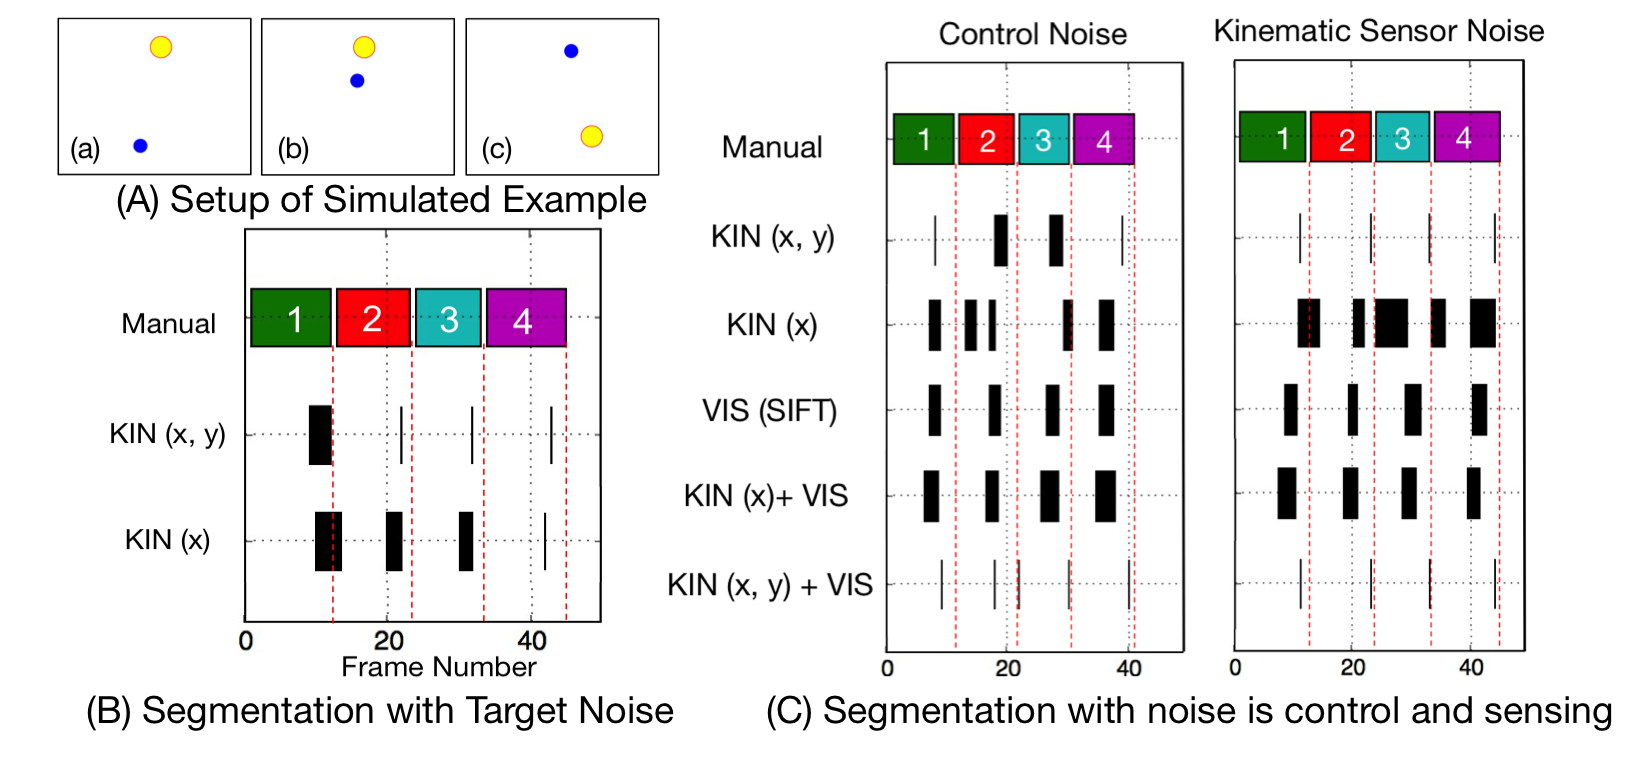
\includegraphics[width=0.8\linewidth]{figures/toyEx}
\caption{The figure shows a simulated example with a robot in blue and target in yellow. The robot moves to the target and a new target appears. In each episode, we have 4 targets in these experiments and each algorithm run uses 5 episodes. The first row shows the manual segmentation -- reaching each target. Subsequent rows illustrate learn segmentation without supervision under various combinations of input data.  
Each row is a sequence of transitions represented by blocks. The width of every block represents the confidence interval conveying the length of transition, with some transitions being sharp while others are longer.\todo{flesh out}}
\label{fig:toyEx}
\vspace{-15pt}
\end{figure*}


\subsection{Evaluation Metric}
The proposed problem of discovering structure without labels is posed as an unsupervised clustering problem. 
Even with ground truth, such as hand annotations, the clustering criteria may not match up perfectly.
We present results with both an intrinsic metric and comparison to ground truth labels when available.
The intrinsic metric we us is \textit{Silhouette Score}, which is defined as,  \vspace{-5pt}
\[ S(i) = \frac{b(i) - a(i)}{max\{a(i), b(i)\},}
\]
where $a(i)$ is defined the average dissimilarity of point $i$ to a cluster $C_j$ as the average of the distance from $i$ to points in $C_j$, and $b(i)$ is defined as minimum mean dissimilarity of point $i$ to cluster $C_k,\ k\neq j$. We can interpret $a(i)$ as the quality of intra-cluster fit, hence a smaller number is better. Similarly, $b(i)$ can be interpreted as inter-cluster fit quality, with higher values deemed better. 
Silhouette Score for each data point is bounded in $[-1, 1]$. Average of $S(i)$ over entire data, measures clustering quality, while average $S(i)$ over all data of a cluster measures density of that cluster. 
We use the mean Silhouette Score over all data for choice of featurization schemes and algorithm evaluation.

For ground truth comparison, we use the \textit{Dynamic Time Warping} distance  between time-steps for transitions and labelled transitions. We normalize it by the temporal length of each example. This metric captures the total error in alignment of predicted transitions to transitions in manual labels. 


\begin{table}[bht!]
\centering
\caption{Evaluation of visual featurization schemes on Suturing}
\label{tab:visual}
\resizebox{\linewidth}{!}{% put in textwidth
\begin{tabular}{l|l|l|l}
\hline
\rowcolor[HTML]{CBCEFB} 
                 & \multicolumn{1}{c|}{CCA}           & \multicolumn{1}{c|}{GRP}          & \multicolumn{1}{c}{PCA}           \\ \hline \hline
SIFT             &          -     &        -     & -0.113$\pm$0.016 \\ %\hline
\rowcolor[HTML]{E0E0E0} 
AlexNet conv3    & -0.013$\pm$0.012 & 0.117$\pm$0.035 & 0.200$\pm$0.024 \\ %\hline 
AlexNet conv4    & -0.025$\pm$0.009 & 0.135$\pm$0.013 & 0.213$\pm$0.007  \\ %\hline
\rowcolor[HTML]{E0E0E0} 
AlexNet pool5    & -0.029$\pm$0.023 & 0.129$\pm$0.016 & 0.197$\pm$0.009  \\ %\hline
VGG conv5\_3     & -0.012$\pm$0.025 & 0.141$\pm$0.010 & \textbf{0.273$\pm$0.018}  \\ %\hline
\rowcolor[HTML]{E0E0E0} 
VGG LCD-VLAD     & 0.046$\pm$0.020  & 0.012$\pm$0.002 & 0.068$\pm$0.023  \\ %\hline
AlexNet LCD-VLAD & 0.068$\pm$0.035  & 0.033$\pm$0.001 & -0.063$\pm$0.053 \\
\hline
\end{tabular}
}
\vspace{-15pt}
\end{table}

\subsection{Evaluation of Visual Featurization}
We first describe our experimental evaluation of the visual featurization by varying different visual featurization parameters.

\begin{figure}[b!]
\centering
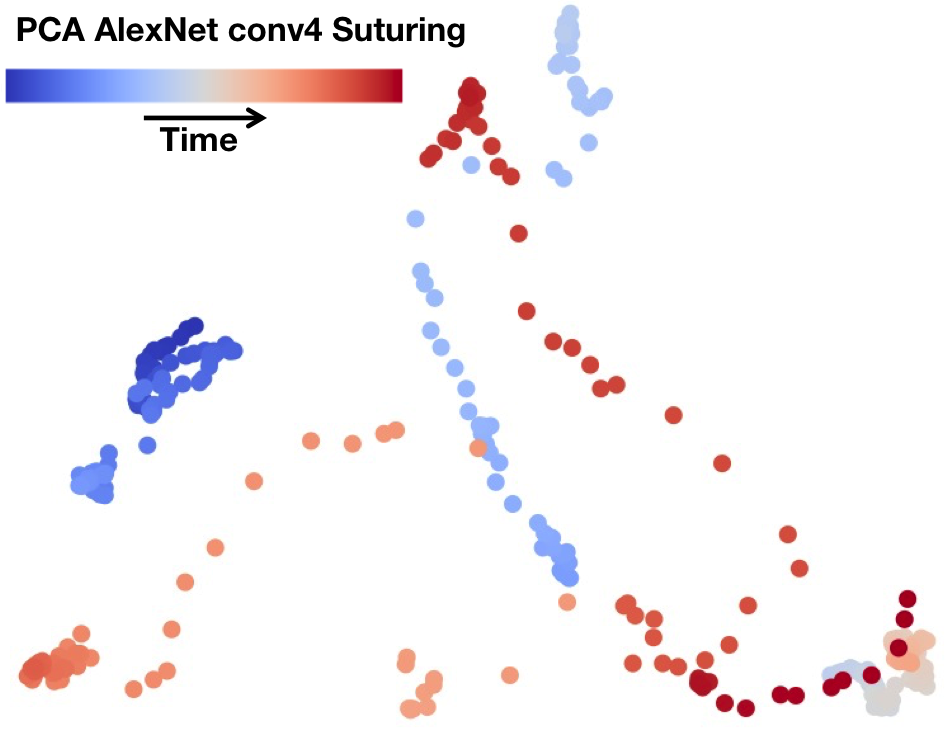
\includegraphics[width=0.7\linewidth]{figures/pca_conv4.png}
\caption{The figure visualizes the PCA projection of 64,896 dimensional output from \texttt{conv4} of the Alexnet for a sub-sequence of the suturing task video sub-sampled at 10 fps. The points are colored according to time from blue to red. We note that the visual features follow a smooth trajectory even in the high dimensional visual space.   \label{fig:imgtraj}}
\vspace{-10pt}
\end{figure}


\subsubsection{Local Linearity of Visual Features}
In our first experiment, we explore whether the transitions state clustering model, orginally derived for locally linear dynamical, is still justified for the augmented state $\binom{k(t)}{z(t)}$.
In Figure \ref{fig:imgtraj}, for a single trajectory from one of our experimental datasets, we plot a 2D PCA visualization of the features from convolutional layer (\texttt{conv4}) of the pre-trained AlexNet architecture. We use a sub-sequence of the full task and sub-sample the data at 10 fps and for each frame, we add a point to the visualization, illustrating the trajectory in feature space. It is worth noting that the visual features follow a smooth trajectory even in the high dimensional visual space, supporting the assumptions of local linearity made by our model for identifying transitions.


\subsubsection{Encoding, Dimensionality Reduction, and Architecture}

